\chapter{Air Separation Technology}
\label{chp:airsep}
There are several ways besides cryogenic air separation to produce highly pure liquid or gaseous
nitrogen and oxygen. In this chapter different competing technologies and their main field of
applications will be discussed. The mainly used technologies asides from the cryogenic process 
are pressure swing adsorption (PSA) as well as membrane processes the so called gas permeation (GP). 

\reffig{fig:tech_compar} illustrates the most economically viable processes depending on product
purity and product stream volume. It is important to remember, that PSA and GP processes exclusively produce 
gaseous products whereas cryogenic air separation may yield liquid or gaseous product streams. 
It can be seen, newer air separation processes cannot supply the high quality or quantity of the cryogenic 
process. Due to that cryogenic air separation is thought to be the main supplier of highly pure gases in 
industrial quantities for years to come \addref.
 
\begin{figure}
	\begingroup%
  \makeatletter%
    \setlength{\unitlength}{1cm}%
  \makeatother%
  \begin{picture}(17, 7)%	
    \scriptsize
    \put(2,1){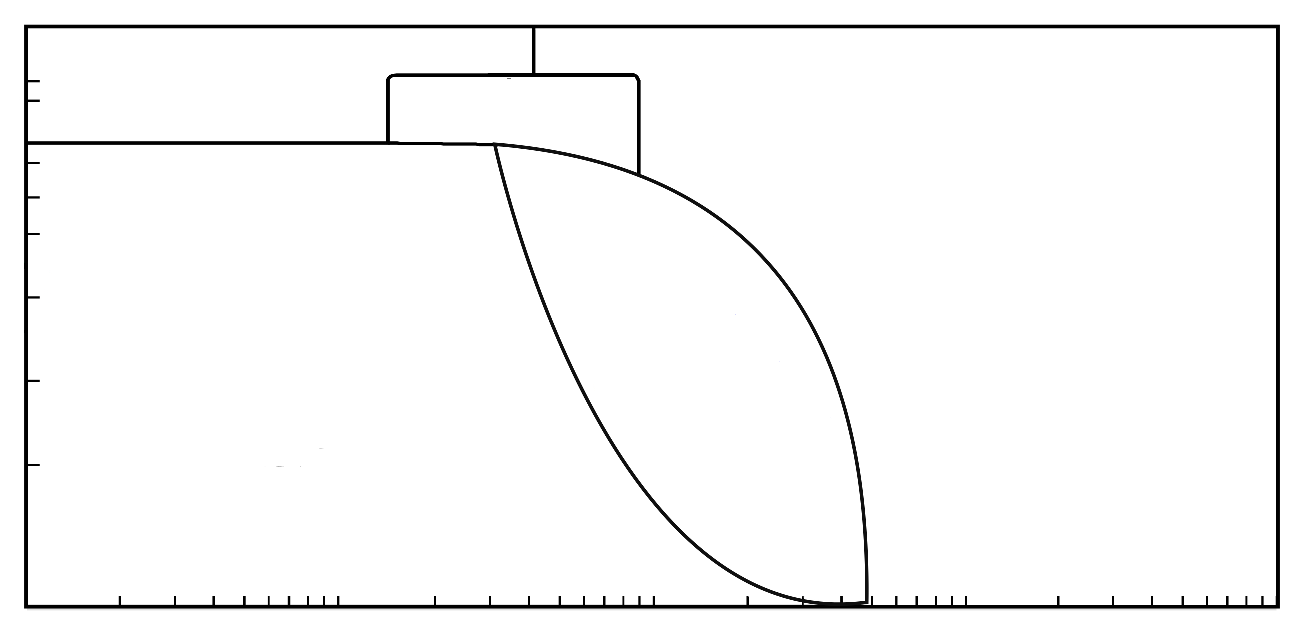
\includegraphics[width=13cm]{Pictures/tech_comp_graph.eps}}%
    \put(8.5, 0.1){\color[rgb]{0,0,0}\makebox(0,0)[c]{\smash{\normalsize{product stream $[\frac{m^3_{STP}}{h}]$}}}}%
    \put(0.6, 4){\color[rgb]{0,0,0}\rotatebox{90}{\makebox(0,0)[c]{\smash{\normalsize{$N_2$-purity $x_{N_2, Ret}$ $[\%]$}}}}}%
    \put(1.9, 0.65){\color[rgb]{0,0,0}\makebox(0,0)[l]{\smash{$10$}}}%
    \put(5.15, 0.65){\color[rgb]{0,0,0}\makebox(0,0)[l]{\smash{$10^2$}}}%
    \put(8.35, 0.65){\color[rgb]{0,0,0}\makebox(0,0)[l]{\smash{$10^3$}}}%
    \put(11.55, 0.65){\color[rgb]{0,0,0}\makebox(0,0)[l]{\smash{$10^4$}}}%
    \put(14.75, 0.65){\color[rgb]{0,0,0}\makebox(0,0)[l]{\smash{$10^5$}}}%
    \put(1.85, 1){\color[rgb]{0,0,0}\makebox(0,0)[r]{\smash{$95$}}}%
    \put(1.85, 2.45){\color[rgb]{0,0,0}\makebox(0,0)[r]{\smash{$97$}}}%
    \put(1.85, 3.325){\color[rgb]{0,0,0}\makebox(0,0)[r]{\smash{$98$}}}%
    \put(1.85, 4.15){\color[rgb]{0,0,0}\makebox(0,0)[r]{\smash{$99$}}}%
    \put(1.85, 4.8){\color[rgb]{0,0,0}\makebox(0,0)[r]{\smash{$99.5$}}}%
    \put(1.85, 5.2){\color[rgb]{0,0,0}\makebox(0,0)[r]{\smash{$99.9$}}}%
    \put(1.85, 5.55){\color[rgb]{0,0,0}\makebox(0,0)[r]{\smash{$99.95$}}}%
    \put(1.85, 6.1){\color[rgb]{0,0,0}\makebox(0,0)[r]{\smash{$99.99$}}}%
    \put(1.85, 6.4){\color[rgb]{0,0,0}\makebox(0,0)[r]{\smash{$99.999$}}}%
    \put(1.85, 6.4){\color[rgb]{0,0,0}\makebox(0,0)[r]{\smash{}}}%
    \put(5,3){\color[rgb]{0,0,0}\normalsize{\CM{membrane processes / \\ gas permeation}}}%
    \put(8.9,3.7){\color[rgb]{0,0,0}\normalsize{\CM{PSA}}}%
    \put(7,6.20){\color[rgb]{0,0,0}\scriptsize{\CM{membrane \& \\ post oxidation}}}%
    \put(4,6.5){\color[rgb]{0,0,0}\normalsize{\CM{cryogenic processes \\ (liquid)}}}%
    \put(12,5.5){\color[rgb]{0,0,0}\normalsize{\CM{cryogenic processes \\ (gaseous)}}}%
  \end{picture}%
\endgroup%

	\caption{Comparison of Air Separation Technologies.}
	\label{fig:tech_compar}
	\todoil{}{addref: http://dx.doi.org/10.1016/0376-7388(93)E0193-N}
\end{figure}

\section{Membrane Processes}
\label{sec:membrane}
\todo[inline]{find paper: DOI: 10.1002/cite.330480804}
The separation of mixed gases by membrane process is called gas permeation. Its main strength 
in comparison with alternative processes are the low energy consumption and the possibility to 
produce flexible mobile units. As mentioned before it is not however capable of producing high
quantity highly pure product streams. As \reffig{fig:tech_compar} illustrates the main application 
for the gas permeation process are moderate product streams at intermediate purities.   

\begin{figure}
	\center
	
\begingroup%
  \makeatletter%
    \setlength{\unitlength}{1cm}%
  \makeatother%
  \begin{picture}(13, 3)%	
    \put(0,0){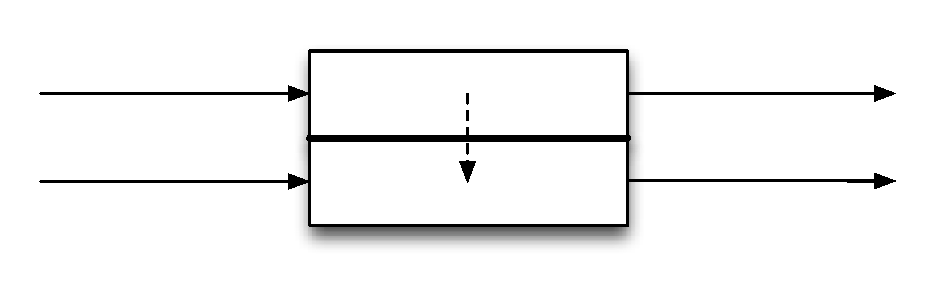
\includegraphics[width=13cm]{Pictures/gas_permeation.eps}}%
    \put(2.3, 1.15){\color[rgb]{0,0,0}\makebox(0,0)[c]{\smash{sweep}}}%
     \put(2.3, 2.40){\color[rgb]{0,0,0}\makebox(0,0)[c]{\smash{feed}}}%
     \put(10.7, 1.15){\color[rgb]{0,0,0}\makebox(0,0)[c]{\smash{retentate}}}%
     \put(10.7, 2.40){\color[rgb]{0,0,0}\makebox(0,0)[c]{\smash{permeate}}}%
  \end{picture}%
\endgroup%

	\caption{Gas permeation process.}
	\label{fig:gas_permeation} 
\end{figure}


\section{Pressure Swing Adsorbtion}
\label{sec:psa}
